\chapter{A Formal Approach to Groups}
\label{chapter:formal_groups}
\thispagestyle{empty}

In this chapter we finally introduce the formal definition of a group.  From this point on, our focus will shift from developing intuition to studying the abstract properties of groups.  However, we should not abandon the intuition we have gained.  As we progress, your intuitive understanding of groups will continue to improve and you should rely on this understanding as you try to make sense of the notions that follow.  There has been plenty of intentional foreshadowing, so expect to revisit concepts you've already encountered.  We'll also encounter plenty of new stuff, too.

It is important to point out that things are about to get quite a bit more difficult for most of you.  Be patient and persistent!

\begin{section}{Binary Operations}
After learning to count as a child, you likely learned how to add, subtract, multiply, and divide with natural numbers.  Loosely speaking, these operations are examples of binary operations since we are combining two objects to obtain a single object.  More formally, we have the following definition.

\begin{definition}
A \textbf{binary operation} $*$ on a set $A$ is a function from $A\times A$ into $A$.  For each $(a,b)\in A\times A$, we denote the element $*(a,b)$ via $a*b$.
\end{definition}

\begin{remark}
Don't misunderstand the use of $*$ in this context.  We are not implying that $*$ is the ordinary multiplication of real numbers that you are familiar with.  We use $*$ to represent a generic binary operation.  
\end{remark}

\begin{remark}
Notice that since the codomain of a binary operation on a set $A$ is $A$, binary operations require that we yield an element of $A$ when combining two elements of $A$.  In this case, we say that $A$ is \textbf{closed} under $*$.  Binary operations have this closure property by definition.  Also, since binary operations are functions, any attempt to combine two elements from $A$ should result in a \emph{unique} element of $A$.  In this case, we say that $*$ is \textbf{well-defined}.  Moreover, since the domain of $*$ is $A\times A$, it must be the case that $*$ is defined for \emph{all} pairs of elements from $A$.
\end{remark}

\begin{example}
Examples of binary operations include $+$ (addition), $-$ (subtraction), and $\cdot$ (multiplication) on the real numbers.  However, $\div$ (division) is not a binary operation on the set of real numbers because all elements of the form $(a,0)$ are not in the domain $\mathbb{R}\times \mathbb{R}$ since we cannot divide by 0.  Yet, $\div$ is a suitable binary operation on $\mathbb{R}\setminus \{0\}$.
\end{example}

\begin{example}
Let $C$ be the set of continuous functions from $\mathbb{R}$ to $\mathbb{R}$.  Then $\circ$ (function composition) is a binary operation on $C$.
\end{example}

\begin{example}
Consider the 6 actions of $D_3$.  The composition of these actions is a binary operation on $D_3$.  In fact, composition of actions for each of the groups that we have seen is a binary operation on the given group.  Notice that we never used a symbol for these binary operations, but rather used juxtaposition (i.e., $ab$ is the juxtaposition of $a$ and $b$).
\end{example}

\begin{example}
Let $M_{2\times 2}(\mathbb{R})$ be the set of $2\times 2$ matrices with real number entries.  Then matrix multiplication is a binary operation on $M_{2\times 2}(\mathbb{R})$.
\end{example}

\begin{exercise}
Explain why composition of spins is not a binary operation on the set of allowable spins in $\Spin_{3\times 3}$.
\end{exercise}

\begin{exercise}
Let $M(\mathbb{R})$ be the set of matrices (of any size) with real number entries.  Is matrix addition a binary operation on $M(\mathbb{R})$?  How about matrix multiplication?
\end{exercise}

\begin{exercise}
Determine whether $\cup$ (union) and $\cap$ (intersection) are binary operations on $\mathcal{P}(\mathbb{Z})$ (i.e., the power set of the integers).
\end{exercise}

\begin{exercise}
Consider the closed interval $[0,1]$ and define $*$ on $[0,1]$ via $a*b=\mathrm{min}\{a,b\}$ (i.e., take the minimum of $a$ and $b$).  Determine whether $*$ is a binary operation on $[0,1]$.
\end{exercise}

Some binary operations have additional properties.

\begin{definition}
Let $A$ be a set and let $*$ be a binary operation on $A$.
\begin{enumerate}
\item We say that $*$ is \textbf{associative} if and only if $(a*b)*c=a*(b*c)$ for all $a,b,c\in A$.
\item We say that $*$ is \textbf{commutative} if and only if $a*b=b*a$ for all $a,b\in A$.
\end{enumerate}
\end{definition}

\begin{exercise}
Provide at least one example of a binary operation and the corresponding set that is commutative.  How about not commutative?
\end{exercise}

\begin{theorem}
Let $A$ be a set and let $F$ be the set of functions from $A$ to $A$.  Then function composition is an associative binary operation on $F$.
\end{theorem}

When the set $A$ is finite, we can represent a binary operation on $A$ using a table in which the elements of the set are listed across the top and the left side (in the same order).  The entry in the $i$th row and $j$th column of the table represents the output of combining the element that labels the $i$th row with the element that labels the $j$th column (order matters).

\begin{example}\label{example:table}
Consider the following table.
\begin{center}
\begin{tabu}{c|[2pt]c|c|c}
$*$ & $a$ & $b$ & $c$ \\ \tabucline[2pt]{-}
$a$ & $b$ & $c$ & $b$ \\
\hline $b$ & $a$ & $c$ & $b$  \\
\hline $c$ & $c$ & $b$ & $a$
\end{tabu}
\end{center}
This table represents a binary operation on the set $A=\{a,b,c\}$.  In this case, $a*b=c$ while $b*a=a$.  This shows that $*$ is not commutative.
\end{example}

\begin{exercise}
What property must a table for a binary operation have in order for the operation to be commutative?
\end{exercise}

\begin{exercise}\label{exer:table_missing_entries}%Exercise 1.2.6 in Fraleigh
Fill in the missing entries in the following table so that $*$ defines an associative binary operation on $\{a,b,c,d\}$.
\begin{center}
\begin{tabu}{c|[2pt]c|c|c|c}
    $*$ & $a$ & $b$ & $c$ & $d$ \\\tabucline[2pt]{-}
    $a$ & $a$ & $b$ & $c$ & $d$ \\\hline
    $b$ & $b$ & $a$ & $c$ & $d$ \\\hline
    $c$ & $c$ & $d$ & $c$ & $d$ \\\hline
    $d$ &  &  & & 
\end{tabu}
\end{center}
\end{exercise}

\end{section}

\begin{section}{Groups}
Without further ado, here is our official definition of a group.

\begin{definition}\label{def:group}
A group $(G,*)$ is a set $G$ together with a binary operation $*$ such that the following axioms hold.
\begin{description}
\item[Axiom 0.] The set $G$ is closed under $*$.
\item[Axiom 1.] The operation $*$ is associative.
\item[Axiom 2.] There is an element $e\in G$ such that for all $g\in G$, $e*g=g*e=g$.  We call $e$ the \textbf{identity}.
\item[Axiom 3.] Corresponding to each $g\in G$, there is an element $g'\in G$ such that $g*g'=g'*g=e$.  In this case, $g'$ is called the \textbf{inverse} of $g$, which we shall denote as $g^{-1}$.
\end{description}
\end{definition}

\begin{remark}
A few comments are in order.
\begin{enumerate}
\item Notice that a group has two parts to it, namely, a set and a binary operation.  For simplicity, if $(G,*)$ is a group, we will often refer to $G$ as being the group.  However, you must remember that the binary operation is part of the structure.
\item Axiom 2 forces $G$ to be nonempty.
\item In the generic case, even if $*$ is not actually multiplication, we will refer to $a*b$ as the product of $a$ and $b$.
\item We are not requiring $*$ to be commutative.  If $*$ is commutative, then we say that $G$ is \textbf{abelian}\footnote{Commutative groups are called abelian in honor of the Norwegian mathematician Niels Abel (1802--1829).} (or \textbf{commutative}).
\end{enumerate}
\end{remark}

\begin{exercise}
Explain why Axiom 0 is unnecessary.
\end{exercise}

At this time, we have two definitions of a group.  The first one was intended to provide an intuitive introduction and Definition~\ref{def:group} provides a rigorous mathematical definition.  We should confirm that these two definitions are in fact compatible.

\begin{exercise}
Compare and contrast our two definitions of a group.  How do the rules and axioms match up?
\end{exercise}

\begin{exercise}
Quickly verify that $\Spin_{1\times 3}$, $S_2$, $R_4$, $D_3$, $D_4$, $V_4$, and $Q_8$ are groups under composition of actions.
\end{exercise}

\begin{exercise}
Determine whether each of the following are groups.  If the pair is a group, determine whether it is abelian and identify the identity.  Explain your answers.
\begin{enumerate}
\item[(a)] $(\mathbb{Z},+)$
\item[(b)] $(\mathbb{N},+)$
\item[(c)] $(\mathbb{Z},\cdot)$
\item[(d)] $(\mathbb{R},+)$
\item[(e)] $(\mathbb{R},\cdot)$
\item[(f)] $(\mathbb{R}\setminus \{0\},\cdot)$
\item[(g)] $(M_{2\times 2}(\mathbb{R}),+)$
\item[(h)] $(M_{2\times 2}(\mathbb{R}),*)$, where $*$ is matrix multiplication.
\item[(i)] $(\{a,b,c\},*)$, where $*$ is the operation determined by the table in Example~\ref{example:table}.
\item[(j)] $(\{a,b,c,d\},*)$, where $*$ is the operation determined by the table in Exercise~\ref{exer:table_missing_entries}.
\end{enumerate}
\end{exercise}

Notice that in Axiom 2 of Definition~\ref{def:group}, we said \emph{the} identity and not \emph{an} identity.  Implicitly, this implies that the identity is unique.

\begin{theorem}\label{thm:unique_id}
Let $G$ be a group with binary operation $*$.  Then there is a unique identity element in $G$.  That is, there is only one element $e$ in $G$ such that $g*e=e*g=g$ for all $g\in G$.
\end{theorem}

The following theorem is crucial for proving many theorems about groups.

\begin{theorem}[Cancellation Law]
Let $(G,*)$ be a group and let $g,x,y\in G$.  Then $g*x=g*y$ if and only if $x=y$.  Similarly, $x*g=y*g$ if and only if $x=y$.\footnote{You only need to prove one of these statements as the proof of the other is symmetric.}
\end{theorem}

\begin{exercise}
Show that $(\mathbb{R},\cdot)$ fails the Cancellation Law (confirming the fact that it is not a group).
\end{exercise}

\begin{corollary}
Let $G$ be a group with binary operation $*$.  Then each $g\in G$ has a unique inverse.
\end{corollary}

\begin{theorem}\label{thm:unique_soln}
Let $(G,*)$ be a group and let $g,h\in G$.  Then the equations $g*x=h$ and $y*g=h$ have unique solutions for $x$ and $y$ in $G$.  
\end{theorem}

While proving the previous few theorems, hopefully one of the things you realized is that you can multiply both sides of a group equation by the same element but that you have to do it on the same side of each half.  That is, since a group may or may not be abelian, if I multiply one side of an equation on the left by a group element, then we must multiply the other side of the equation on the left by the same group element.

Despite the fact that a group may or may not be abelian, if one product is equal to the identity, then reversing the order yields the same result.

\begin{theorem}
Let $G$ be a group with binary operation $*$.  If $g*h=e$, then $h*g=e$.
\end{theorem}

The upshot of the previous theorem is if we have a ``left inverse" then we automatically have a ``right inverse" (and vice versa).

The next theorem should not be surprising.

\begin{theorem}
Let $(G,*)$ be a group and let $g\in G$.  Then $(g^{-1})^{-1}=g$.
\end{theorem}

\begin{definition}
Let $(G,*)$ be a group and let $g\in G$.  Then for $n\in \mathbb{N}$, we define
\[
g^n=\underbrace{g*g*\cdots *g}_{n\text{ factors}}
\]
and
\[
g^{-n}=\underbrace{g^{-1}*g^{-1}*\cdots *g^{-1}}_{n\text{ factors}}.
\]
Moreover, we define $g^0=e$.
\end{definition}

The good news is that the rules of exponents you are familiar with still hold for groups.

\begin{theorem}
Let $(G,*)$ be a group and let $g\in G$.  If $n\in\mathbb{Z}$, then:
\begin{enumerate}
\item $g^n*g^m=g^{n+m}$,
\item $(g^n)^{-1}=g^{-n}$.
\end{enumerate}
\end{theorem}

\end{section}

\begin{section}{Group Tables}
Recall that we could represent a binary operation on a finite set using a table.  Since groups have binary operations at their core, we can represent a finite group (i.e., a group with finitely many elements) using a table, called a \textbf{group table}. For example, the following is a group table for $V_4$.

\begin{center}
\begin{tabu}{c|[2pt]c|c|c|c}
$*$ & $e$ & $v$ & $h$ & $vh$ \\ \tabucline[2pt]{-}
$e$ & $e$ & $v$ & $h$ & $vh$ \\
\hline $v$ & $v$ & $e$ & $vh$ & $h$  \\
\hline $h$ & $h$ & $vh$ & $e$ & $v$\\
\hline $vh$ & $vh$ & $h$ & $v$ & $e$
\end{tabu}
\end{center}

\begin{exercise}
Verify that $V_4$ is an abelian group.  What feature of the group table makes this clear?
\end{exercise}

Notice that above I said, ``a group table for $V_4$" and not ``the group table."  The reason for this is that if we chose a different order of the elements (e.g., swap rows 1 and 4---which swaps columns 1 and 4, as well), then the table would look slightly different.  Also, if we had chosen a different generating set, then the names of the elements would look different.  Regardless, the table still captures the same information about the binary operation.

\begin{exercise}
Create group tables for the following groups: $S_2$, $R_3$, $R_4$, $D_3$, $S_3$, $D_4$, and $Q_8$.  Which groups are abelian?
\end{exercise}

Perhaps you noticed when creating the tables above that each element of the group appeared exactly once in each row and column, respectively.  This is true, in general.  Use Theorem~\ref{thm:unique_soln}, to prove the following theorem.

\begin{theorem}
Let $(G,*)$ be a finite group.  Then each element of $G$ appears exactly once in each row and each column, respectively, in any group table for $G$.
\end{theorem}

We can also use tables to define groups.  For example, consider the following table on the set $A=\{e,a,b,c\}$.

\begin{center}
\begin{tabu}{c|[2pt]c|c|c|c}
$*$ & $e$ & $a$ & $b$ & $c$ \\ \tabucline[2pt]{-}
$e$ & $e$ & $a$ & $b$ & $c$ \\
\hline $a$ & $a$ & $e$ & $c$ & $b$  \\
\hline $b$ & $b$ & $c$ & $e$ & $a$\\
\hline $c$ & $c$ & $b$ & $a$ & $e$
\end{tabu}
\end{center}

\noindent Is this a table for a group?  First, we see that the binary operation determined by the table is closed.  Second, we see that $e$ is acting as the identity.  Since every row and column has the identity element $e$ appearing, we know that every element has an inverse (do you see why that follows?).  The only thing left to check is associativity.  Imagine for a moment what this entails.  It's messy right?!  And this is only for a group of order 4.

Thankfully, we can rely on some prior knowledge to help out with associativity.  It turns out that if you look closely, the group table for $V_4$ looks the ``same" as the table above.  What do we mean by ``same" here?  The names for elements are different (except for $e$), but 
\begin{quotation}
\emph{the product of corresponding elements yields the corresponding result.}
\end{quotation}
To see what I mean, let's color both tables with white, red, blue, and green in such a way that each element corresponds to a unique color.  If we choose our colors wisely, it is easy to see that both tables have the same structure.

\begin{center}
\begin{tabu}{c|[2pt]c|c|c|c}
$*$ & $e$ & \cellcolor{red}$v$ & \cellcolor{blue}$h$ & \cellcolor{green}$vh$ \\ \tabucline[2pt]{-}
$e$ & $e$ & \cellcolor{red}$v$ & \cellcolor{blue}$h$ & \cellcolor{green}$vh$ \\
\hline \cellcolor{red}$v$ & \cellcolor{red}$v$ & $e$ & \cellcolor{green}$vh$ & \cellcolor{blue}$h$  \\
\hline \cellcolor{blue}$h$ & \cellcolor{blue}$h$ & \cellcolor{green}$vh$ & $e$ & \cellcolor{red}$v$\\
\hline \cellcolor{green}$vh$ & \cellcolor{green}$vh$ & \cellcolor{blue}$h$ & \cellcolor{red}$v$ & $e$
\end{tabu}
\hspace{1cm}
\begin{tabu}{c|[2pt]c|c|c|c}
$*$ & $e$ & \cellcolor{red}$a$ & \cellcolor{blue}$b$ & \cellcolor{green}$c$ \\ \tabucline[2pt]{-}
$e$ & $e$ & \cellcolor{red}$a$ & \cellcolor{blue}$b$ & \cellcolor{green}$c$ \\
\hline \cellcolor{red}$a$ & \cellcolor{red}$a$ & $e$ & \cellcolor{green}$c$ & \cellcolor{blue}$b$  \\
\hline \cellcolor{blue}$b$ & \cellcolor{blue}$b$ & \cellcolor{green}$c$ & $e$ & \cellcolor{red}$a$\\
\hline \cellcolor{green}$c$ & \cellcolor{green}$c$ & \cellcolor{blue}$b$ & \cellcolor{red}$a$ & $e$
\end{tabu}
\end{center}

\noindent Since we already know that $V_4$ is a group, we know that the binary operation for $V_4$ is associative.  

\begin{exercise}
Explain why the discussion above implies that the binary operation determined by the table on the right above must be associative.  Have we shown that $(A,*)$ is a group?
\end{exercise}

It is important to point out that if we had not chosen our colors wisely, then perhaps the colorings of the two tables would not agree.  Moreover, if we had made the same color choices for elements, but then rearranged columns and rows of one table, the colorings of the two tables would not agree.  This doesn't imply anything.  The point is whether we \emph{can} get the tables to match.

\begin{exercise}
Draw the Cayley diagram for $(A,*)$ with generators $a$ and $b$.  Explain why this implies that $V_4$ and $A$ (under their respective binary operations) are isomorphic.  
\end{exercise}

\begin{exercise}
Is it possible to color the group table for $R_4$ so that it matches the coloring of $V_4$?  Explain your answer.
\end{exercise}

\begin{problem}\label{prob:iso_same_group_table}
Let $(G,*)$ and $(G',\circ)$ be two finite groups.  Suppose we can arrange the rows and columns and color elements in such a way that the colorings for the two group tables agree.  Explain why this implies that the two groups are isomorphic.
\end{problem}

\begin{problem}
Suppose we have a table for $(G,*)$, where $G$ is finite.  Further suppose that (i) there is an identity element, and (ii) every element appears exactly once in each row and column, respectively.  Explain why the only thing we need to verify in order for $(G,*)$ to be a group is that $*$ is associative.
\end{problem}

\begin{problem}%Exercise 4.18 in VGT
Suppose that $(G,*)$ is a group.  Theorem~\ref{thm:unique_id} guarantees that there is a unique identity in $G$.  When creating the group table for $G$, what goes wrong if you try to include two different identity elements?
\end{problem}

Consider the class of all possible groups.  It turns out that ``isomorphic" ($\cong$) determines an equivalence relation.  That is, under this relation two groups are related if and only if they are isomorphic.  We'll prove this formally later when we have a more rigorous definition of isomorphic.

\begin{problem}
Explain why all groups with a single element are isomorphic.
\end{problem}

In this case, we say that ``up to isomorphism" there is only one group with a single element.

\begin{problem}
Consider a group $(G,*)$ of order 2.  Suppose that $G=\{e,a\}$.  Complete the following group table for $G$.

\begin{center}
\begin{tabu}{c|[2pt]c|c}
$*$ & $e$ & $a$ \\ \tabucline[2pt]{-}
$e$ &  &  \\
\hline $a$ &  & 
\end{tabu}
\end{center}
Explain why every group with 2 elements must be isomorphic to $S_2$.
\end{problem}

The previous problem implies that up to isomorphism, there is only one group of order 2.

\begin{problem}
Consider a group $(G,*)$ of order 3.  Suppose that $G=\{e,a,b\}$.  Complete the following group table for $G$.

\begin{center}
\begin{tabu}{c|[2pt]c|c|c}
$*$ & $e$ & $a$ & $b$ \\ \tabucline[2pt]{-}
$e$ &  &  & \\
\hline $a$ &  & & \\
\hline $b$ &  & &
\end{tabu}
\end{center}
Explain why every group with 3 elements must be isomorphic to $R_3$.
\end{problem}

\begin{problem}
Consider a group $(G,*)$ of order 4.  Suppose that $G=\{e,a,b,c\}$.  Assuming that $e$ is the identity, the first row and first column of the corresponding group table must be completed as follows.

\begin{center}
\begin{tabu}{c|[2pt]c|c|c|c}
$*$ & $e$ & $a$ & $b$ & $c$ \\ \tabucline[2pt]{-}
$e$ &  $e$ & $a$ & $b$ & $c$ \\
\hline $a$ & $a$ & ? & & \\
\hline $b$ & $b$ & & & \\
\hline $c$ & $c$ & & &
\end{tabu}
\end{center}

\noindent The cell with the question mark cannot be filled with an $a$.  So, this entry must be either $e$, $b$, or $c$.  However, it should be easy to see the cases with $b$ and $c$ are symmetric.  Thus, there are two cases: (i) the entry with the question mark is filled with $e$, (ii) the entry with the question mark is (without loss of generality) filled with $b$.  Complete the group table in each of these two cases.  Recall that we've seen two non-isomorphic groups of order 2, namely $R_4$ and $V_4$.  What conclusion can you make about groups of order 4?
\end{problem}

So far we've seen that there are unique groups up to isomorphism of orders 1, 2, and 3, but that there are two groups up to isomorphism of order 4.  A general question we will want to address is, how many groups are there of order $n$?

In a future chapter we will be able to prove that there is only one group up to isomorphism of order 5, namely those groups isomorphic to $R_5$ (i.e., rotation group of a regular pentagon).

We've seen three groups of order 6, namely $R_6$, $D_3$, and $S_3$.  However, $D_3\cong S_3$ (see Problem \ref{prob:D3_iso_S3}) while $R_6$ is not isomorphic to either of these (see Problem \ref{prob:R6_not_iso_D3}).  So, we can conclude that there are at least two groups up to isomorphism of order 6.   But are there others?  It turns out that the answer is yes, but why?

The group $R_7$ is the group of rotations of a regular 7-sided polygon.  This group has order 7.  Are there other groups of order 7 that are not isomorphic to $R_7$? 

We've encountered four groups of order 8, namely $D_4$, $\Spin_{1\times 2}$, $Q_8$, and $R_8$.  Of these, only $D_4$ and $\Spin_{1\times 2}$ are isomorphic.  Thus, there are at least three groups up to isomorphism of order 8.  However, are these the only ones?  It turns out that the answer is no.  What are the missing ones?

\end{section}

\begin{section}{Revisiting Cayley Diagrams and Our Original Definition of a Group}%This section closely mimics Section 6.1 in VGT

Let's begin with a couple exercises.

\begin{exercise}\label{exer:nonregular1}%Exercise 4.16 in VGT
Consider the following diagram that we saw at the end of Chapter~\ref{chapter:cayley_diagrams}.
\begin{center}
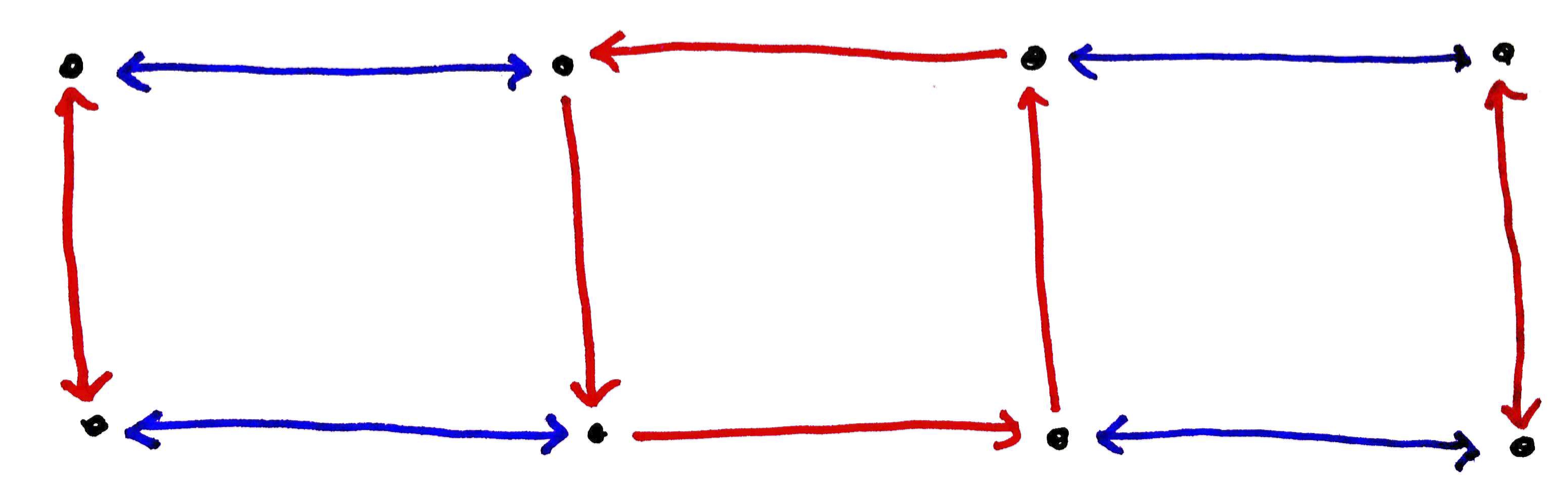
\includegraphics[width=5in]{nonregular.png}
\end{center}
\begin{enumerate}
\item[(a)] Consider Rules 1--4 of our original definition of a group (see Definition~\ref{def:informal_group}).  Does the above diagram satisfy Rules 1--4?
\item[(b)] Try to convert this diagram into a group table.  Does the table represent a group? What goes wrong?
\end{enumerate}
\end{exercise}

\begin{exercise}\label{exer:nonregular2}%Exercise 4.16 in VGT
Consider the following diagram.

\tikzstyle{vert} = [circle, draw, fill=grey,inner sep=0pt, minimum size=4mm]
\tikzstyle{b} = [draw,very thick,blue,stealth-stealth]
\tikzstyle{r} = [draw, very thick, red,-stealth]

\begin{center}
\begin{tikzpicture}[auto]
\node (1) at (0,0) [vert] {};
\node (2) at (2,0) [vert] {};
\node (3) at (4,0) [vert] {};
\node (4) at (6,0) [vert] {};
\node (5) at (0,2) [vert] {};
\node (6) at (2,2) [vert] {};
\node (7) at (4,2) [vert] {};
\node (8) at (6,2) [vert] {};

\path[b] (1) to (5);
\path[b] (2) to (6);
\path[b] (3) to (8);
\path[b] (4) to (7);

\path[r] (1) to (2);
\path[r] (2) to (3);
\path[r] (3) to (4);
\path[r] (4) to [bend left] (1);
\path[r] (5) to (6);
\path[r] (6) to (7);
\path[r] (7) to (8);
\path[r] (8) to [bend right] (5);
\end{tikzpicture}
\end{center}
\begin{enumerate}
\item[(a)] Does the above diagram satisfy Rules 1--4 of Definition~\ref{def:informal_group}?
\item[(b)] Try to convert this diagram into a group table.  Does the table represent a group? What goes wrong?
\end{enumerate}
\end{exercise}

As the previous two exercises indicate, the moral of the story is that our original intuitive definition of a group has a weakness.  It does not agree with our formal definition of a group given in Definition~\ref{def:group}.  Let's see if we can figure out what goes wrong.

Consider the Cayley diagram for $D_3$ with generators $r$ and $s$.

\tikzstyle{vert} = [circle, draw, fill=grey,inner sep=0pt, minimum size=8mm]
\tikzstyle{h} = [draw,very  thick, blue,stealth-stealth]
\tikzstyle{r} = [draw, very thick, red,-stealth]

\begin{center}
\begin{tikzpicture}[scale=.75,auto]
\node (e) at (90:2) [vert] {$e$};
\node (r) at (-30:2) [vert] {$r$};
\node (rr) at (210:2) [vert] {$r^2$};
\node (h) at (90:4) [vert] {$s$};
\node (hr) at (210:4) [vert] {$rs$};
\node (hrr) at (-30:4) [vert] {$r^2s$};
\draw [r] (e) to [bend left] (r);
\draw [r] (r) to [bend left] (rr);
\draw [r] (rr) to [bend left] (e);
\draw [r] (h) to [bend right] (hr);
\draw [r] (hr) to [bend right] (hrr);
\draw [r] (hrr) to [bend right] (h);
\draw [h] (e) to (h);
\draw [h] (r) to (hrr);
\draw [h] (rr) to (hr);
\end{tikzpicture}
\end{center}

\noindent Notice that we labeled the lower right corner of the Cayley diagram with the word $r^2s$.  This means that we first followed a blue arrow out of $e$ and then two red arrows.  However, we could also get to this vertex by first doing a red arrow out of $e$ followed by a blue arrow.  So, we could also have labeled this vertex with the word $sr$.  The upshot is that $r^2s=sr$.  These types of group equations are called \textbf{relations}.

We discovered this relation by starting at $e$ and then traveling a sequence of arrows to get to the vertex in the lower right corner.  However, notice that following a blue and then two red arrows is \emph{always} the same as following a red arrow and then a blue arrow regardless of which vertex we start at.  That is, the relation $r^2s=sr$ holds universally across the entire Cayley diagram.

Cayley diagrams for groups will always have this uniform symmetry.  The fancy way of saying this is that Cayley diagrams are \textbf{regular}.  In other words, a diagram is regular if every internal pattern repeats itself throughout the diagram.

\begin{exercise}
Identify two other relations that the above Cayley diagram for $D_3$ exhibits.  Find one that involves both $r^{-1}$ (i.e., following a red arrow backwards) and $s$.  Convince yourself that your relations appear throughout the diagram.
\end{exercise}

\begin{exercise}
Verify that the diagrams in Exercise~\ref{exer:nonregular1} and \ref{exer:nonregular2} are not regular.
\end{exercise}

\begin{problem}
Explain why the Cayley diagram for a group must be regular.
\end{problem}

The discussion and exercises above lead us to conclude that one thing missing from our original intuitive definition of a group is regularity.  It turns out that this is the only thing missing.  That is, if we add the requirement of regularity to our intuitive definition, we could convert it into a rigorous definition that is equivalent to Definition~\ref{def:group}.  However, we won't bother doing this since our intuitive definition served its purpose.

\end{section}

\begin{section}{Revisiting Subgroups}

Back in Section~\ref{sec:intuitive_subgroups}, we introduced the notion of subgroup.  In light of our official definition of a group, we more or less have the same definition as before, but let's restate it here using slightly more formal language.

\begin{definition}
Let $(G,*)$ be a group and let $H$ be a subset of $G$.  Then $H$ is a \textbf{subgroup} of $G$, written $H\leq G$, provided that $H$ is a group in its own right under the binary operation inherited from $G$.
\end{definition}

The phrase ``under the binary operation inherited from $G$" means that to combine two elements in $H$, we should treat the elements as if they were in $G$ and perform $G$'s binary operation.

Recall that Theorems~\ref{thm:trivial_subgroup1} and \ref{thm:trivial_subgroup2} tell us that $\langle e\rangle=\{e\}$ and $G$ are always subgroups of $G$. This is still true even using our official definition of a group.  These two subgroups are referred to as the \textbf{trivial subgroups}\footnote{Some textbooks will refer to $\{e\}$ as being the trivial subgroup and $G$ as the improper subgroup.}.  All other subgroups are called \textbf{nontrivial}.  If $H$ is a nontrivial subgroup of a group $G$, then we may write $H<G$.

Using our unofficial definition of a group, Theorem~\ref{thm:informal_subgroup_criterion} told us that a subset $H$ of a group $G$ was a subgroup if it satisfied Rules 2 and 4.  The theorem below is the analogous statement for our official definition of a group.

\begin{theorem}\label{thm:subgroup_criterion}
Suppose $(G,*)$ is a group and $H$ is a nonempty subset of $G$.  Then $H\leq G$ if and only if (i) for all $h\in H$, $h^{-1} \in H$, as well, and (ii) $H$ is closed under the binary operation of $G$.
\end{theorem}

\begin{exercise}
Consider $(\mathbb{R}^3,+)$, where $\mathbb{R}^3$ is the set of all 3-entry row vectors with real number entries (e.g., $(a,b,c)$ where $a,b,c\in\mathbb{R}$) and $+$ is ordinary vector addition.  It turns out that $(\mathbb{R}^3,+)$ is an abelian group with identity $(0,0,0)$.  
\begin{enumerate}
\item[(a)] Let $H$ be the subset of $\mathbb{R}^3$ consisting of vectors with first coordinate 0.  Is $H$ is a subgroup of $\mathbb{R}^3$?  Prove your answer.
\item[(b)] Let $K$ be the subset of $\mathbb{R}^3$ consisting of vectors whose entries sum to 0.  Is $K$ is a subgroup of $\mathbb{R}^3$?  Prove your answer.
\item[(c)] Construct a subset of $\mathbb{R}^3$ (different from $H$ and $K$) that is \emph{not} a subgroup of $\mathbb{R}^3$.
\end{enumerate}
\end{exercise}

\begin{exercise}\label{exer:nZ}
Consider the group $(\mathbb{Z},+)$ (under ordinary addition).
\begin{enumerate}
\item[(a)] Show that the even integers, written $2\mathbb{Z}:=\{2k:k\in\mathbb{Z}\}$, form a subgroup of $\mathbb{Z}$.
\item[(b)] Show that the odd integers are not a subgroup of $\mathbb{Z}$.
\item[(c)] Show that all subsets of the form $n\mathbb{Z}:=\{nk:k\in\mathbb{Z}\}$ for $n\in\mathbb{Z}$ are subgroups of $\mathbb{Z}$.
\item[(d)] Are there any other subgroups besides the ones listed in part (c)?  Explain your answer.
\end{enumerate}
\end{exercise}

\begin{exercise}
Consider the group of symmetries of a regular octagon.  This group is denoted by $D_8$, where the operation is composition of actions.  The group $D_8$ consists of 16 elements (8 rotations and 8 reflections).  Let $H$ be the subset consisting of the following clockwise rotations: $0^\circ$, $90^\circ$, $180^\circ$, and $270^\circ$.  Determine whether $H$ is a subgroup of $D_8$ and justify your answer.
\end{exercise}

\begin{exercise}
Consider the groups $(\mathbb{R},+)$ and $(\mathbb{R}\setminus\{0\},\cdot)$.  Explain why $\mathbb{R}\setminus\{0\}$ is not a subgroup of $\mathbb{R}$ despite the fact that $\mathbb{R}\setminus\{0\}\subseteq\mathbb{R}$ and both are groups.
\end{exercise}

\begin{theorem}
Suppose $(G,*)$ is a group and let $H,K\leq G$.  Then $H\cap K\leq G$.
\end{theorem}

\begin{problem}
Can we replace intersection with union in the theorem above?  If so, prove the corresponding theorem.  If not, then provide a specific counterexample.
\end{problem}

\begin{theorem}
Suppose $(G,*)$ is a group.  Define
\[
Z(G):=\{z\in G:zg=gz\text{ for all } g\in G\}
\]
(called the \textbf{center} of $G$).  Then $Z(G)$ is an abelian subgroup of $G$.
\end{theorem}

The following definition formalizes Definition~\ref{def:subgroup_gen_by}.

\begin{definition}
Let $(G,*)$ be a group and let $S$ be a nonempty subset of $G$.  Then we define $\langle S\rangle$ to be the set consisting of all possible (finite) products of elements from $S$ and their inverses.  The set $\langle S\rangle$ is called the \textbf{subgroup generated by $S$}.  The elements of $S$ are called \textbf{generators} of $\langle S\rangle$.
\end{definition}

Note that $S$ may be finite or infinite.  Moreover, even if $S$ is finite, $\langle S\rangle$ may be infinite.  Also, it is important to point out that we are not putting any restrictions about efficiency on $S$ in the definition above.  That is, it is possible that some elements are included in $S$ that are not necessary to generate all of the elements of $\langle S\rangle$.

In cases when we know what the elements of $S$ actually are, then we will list them inside the angle brackets without the set braces.  For example, if $S=\{a,b,c\}$, then we will write $\langle a, b, c\rangle$ instead of $\langle \{a,b,c\}\rangle$.  In the special case when $S$ equals a single element, say $S=\{a\}$, then
\[
\langle a\rangle =\{a^n:n\in\mathbb{Z}\},
\]
which is called the \textbf{subgroup generated by $a$}.  

The set $\langle S\rangle$ is called the ``subgroup generated by $S$", so it better be a subgroup!

\begin{theorem}\label{thm:smallest_subgroup_containing_S}
Let $(G,*)$ be a group and let $S\subseteq G$.  Then $\langle S\rangle \leq G$.  Moreover, $\langle S\rangle$ is the smallest subgroup of $G$ containing $S$.
\end{theorem}

\begin{exercise}
In Exercise~\ref{exer:nZ} we introduced the notation $n\mathbb{Z}$.  Write these subgroups in the ``generated by" notation.  That is, find a set $S$ such that $\langle S\rangle =n\mathbb{Z}$.  Can you find more than one way to do it?
\end{exercise}

Every subgroup can be written in the ``generated by" form.  That is, if $H$ is a subgroup of a group $G$, then there always exists a subset $S$ of $G$ such that $\langle S\rangle=H$.  In particular, $\langle H\rangle=H$.

Let's explore a couple of examples.  First, consider the group $R_4$ (where the operation is composition of actions).  What are the subgroups of $R_4$?  Theorems~\ref{thm:trivial_subgroup1} and \ref{thm:trivial_subgroup2} tell use that $\{e\}$ and $R_4$ itself are subgroups of $R_4$.  Are there any others?  Theorem~\ref{thm:subgroup_criterion} tells us that if we want to find other subgroups of $R_4$, we need to find nonempty subsets of $R_4$ that are closed and contain all the necessary inverses.  However, the previous paragraph indicates that we can find all of the subgroups of $R_4$ by forming the subgroups generated by various combinations of elements from $R_4$.  We can certainly be more efficient, but below we list all of the possible subgroups we can generate using subsets of $R_4$.  We are assuming that $r$ is rotation by $90^{\circ}$ clockwise.  As you scan the list, you should take a moment to convince yourself that the list is accurate.
\begin{multicols}{2}
\begin{itemize}
\item[] $\langle e \rangle = \{e\}$
\item[] $\langle r \rangle  = \{e,r,r^2,r^3\}$
\item[] $\langle r^2 \rangle  = \{e.r^2\}$
\item[] $\langle r^3 \rangle  = \{e,r^3,r^2,r\}$
\item[] $\langle e,r \rangle  = \{e,r,r^2,r^3\}$
\item[] $\langle e,r^2 \rangle  = \{e.r^2\}$
\item[] $\langle e,r^3 \rangle  = \{e,r^3,r^2,r\}$
\item[] $\langle r,r^2 \rangle  = \{e,r,r^2,r^3\}$
\item[] $\langle r,r^3 \rangle  = \{e,r,r^2,r^3\}$
\item[] $\langle r,r^2 \rangle  = \{e,r,r^2,r^3\}$
\item[] $\langle r^2,r^3 \rangle  = \{e,r,r^2,r^3\}$
\item[] $\langle e,r,r^2 \rangle  = \{e,r,r^2,r^3\}$
\item[] $\langle e,r,r^3 \rangle  = \{e,r,r^2,r^3\}$
\item[] $\langle e,r^2,r^3 \rangle  = \{e,r,r^2,r^3\}$
\item[] $\langle r,r^2,r^3 \rangle  = \{e,r,r^2,r^3\}$
\item[] $\langle e,r,r^2,r^3 \rangle = \{e,r,r^2,r^3\}$
\end{itemize}
\end{multicols}
Let's make a few observations.  Scanning the list, we see only three distinct subgroups: $\{e\}, \{e,r^2\},\{e,r,r^2,r^3\}$.  Our exhaustive search guarantees that these are the only subgroups of $R_4$.  It is also worth pointing out that if a subset contains either $r$ or $r^3$, then that subset generates all of $R_4$.  The reason for this is that $r$ and $r^3$ are each generators for $R_4$, respectively.  Also, observe that if we increase the size of the subset using an element that was already contained in the subgroup generated by the smaller set, then we don't get anything new.  For example, consider $\langle r^2\rangle=\{e,r^2\}$.  Since $e\in\langle r^2\rangle$, we don't get anything new by including $e$ in our generating set.  We can state this as a general fact.

\begin{theorem}
Let $(G,*)$ be a group and let $a,b,c\in G$.  If $c\in\langle a,b\rangle$, then $\langle a,b\rangle = \langle a,b,c\rangle$.
\end{theorem}

It is important to point out that in the theorem above, we are not saying that $a$ and $b$ are generators for $G$---although this may be the case.  Instead, are simply making a statement about the subgroup $\langle a,b\rangle$, whatever it may be.

Let's return to our example involving $R_4$.  We have three subgroups, namely the two trivial subgroups $\{e\}$ and $R_4$ itself, together with one nontrivial subgroup $\{e,r^2\}$.  Notice that $\{e\}$ is also a subgroup of $\{e,r^2\}$.  We can capture the overall relationship between the subgroups using a \textbf{subgroup lattice}, which we depict below in the case of $R_4$.

\begin{center}
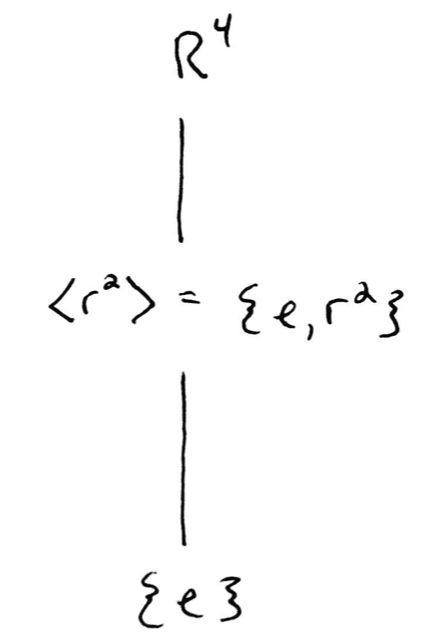
\includegraphics[height=2in]{latticeR4.png}
\end{center}

In general, subgroups of smaller order are towards the bottom of the lattice while larger subgroups are towards the top.  Moreover, an edge between to subgroups means that the smaller set is a subgroup of the larger set.

Let's see what we can do with $V_4=\{e,v,h,vh\}$.  Using an exhaustive search, we find that there are five subgroups:
\begin{itemize}
\item[] $\langle e \rangle = \{e\}$
\item[] $\langle h \rangle  = \{e,h\}$
\item[] $\langle v \rangle  = \{e.v\}$
\item[] $\langle vh \rangle  = \{e,vh\}$
\item[] $\langle v,h \rangle = \langle v,vh\rangle = \langle h, vh\rangle= \{e,v,h,vh\}=V_4$
\end{itemize}
For each subgroup above, we've used minimal generating sets to determine the group.  (Note that minimal generating sets are generating sets where we cannot remove any elements and still obtain the same group.  Two minimal generating sets for the same group do not have to have the same number of generators.)  In this case, we get the following subgroup lattice.

\begin{center}
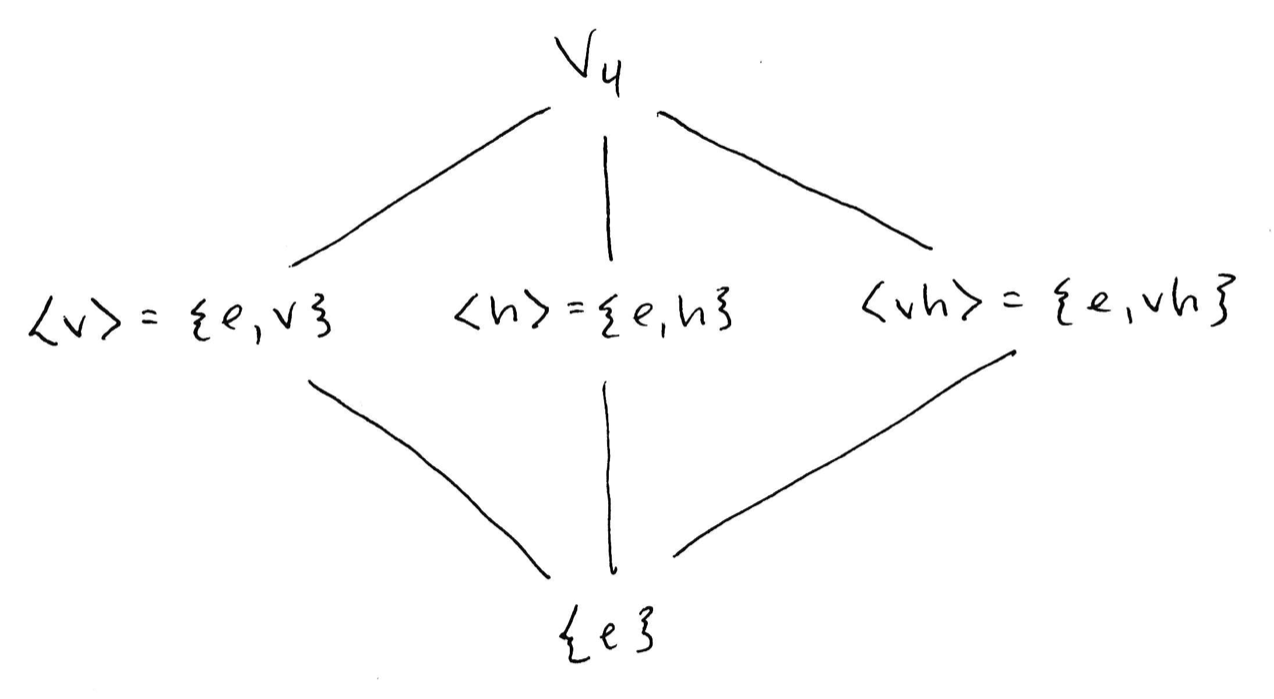
\includegraphics[height=2in]{latticeV4.png}
\end{center}

Notice that there are no edges among $\langle v\rangle, \langle h\rangle$, and $\langle vh\rangle$.  The reason for this is that none of these groups are subgroups of each other.  We already know that $R_4$ and $V_4$ are not isomorphic, but this becomes even more apparent if you compare their subgroup lattices.

\begin{problem}
What claims can be made about the subgroup lattices of two groups that are isomorphic? What claims can be made about the subgroup lattices of two groups that are not isomorphic?  What claims can be made about two groups if their subgroup lattices look nothing alike?  \emph{Hint:} The answers to two of these questions should be obvious, but the answer to the remaining question should be something like, ``we don't have enough information to make any claims."
\end{problem}

In the next few exercises, you are asked to create subgroup lattices.  As you do this, try to minimize the amount of work it takes to come up with all the subgroups.  In particular, I do \emph{not} recommend doing a full brute-force like we did for $R_4$. 

\begin{exercise}
Find all the subgroups of $R_5=\{e,r,r^2,r^3,r^4\}$ (where $r$ is rotation of a regular pentagon by $72^{\circ}$) and then draw the subgroup lattice for $R_5$.
\end{exercise}

\begin{exercise}
Find all the subgroups of $R_6=\{e,r,r^2,r^3,r^4,r^5\}$ (where $r$ is rotation of a regular hexagon by $60^{\circ}$) and then draw the subgroup lattice for $R_6$.
\end{exercise}

\begin{exercise}
Find all the subgroups of $D_3=\{e,r,r^2,s,sr,sr^2\}$ (where $r$ and $s$ are the usual actions) and then draw the subgroup lattice for $D_3$.
\end{exercise}

\begin{exercise}
Find all the subgroups of $D_4=\{e,r,r^2,r^3,s,sr,sr^2,sr^3\}$ (where $r$ and $s$ are the usual actions) and then draw the subgroup lattice for $D_4$.
\end{exercise}

\begin{exercise}
Find all the subgroups of $Q_8=\{1,-1,i,-i,j,-j,k,-k\}$ and then draw the subgroup lattice for $Q_8$.
\end{exercise}

Here are two final problems to conclude this section.

\begin{problem}
Several times we've referred to the fact that some subgroups are visible in a Cayley diagram for the parent group and some subgroups are not.  Suppose $(G,*)$ is a group and let $H\leq G$.  Can you describe a process for creating a Cayley diagram for $G$ that ``reveals" the subgroup $H$ inside of this Cayley diagram?
\end{problem}

\begin{problem}
Suppose $(G,*)$ is a finite group and let $H\leq G$.  Can you describe a process that ``reveals" the subgroup $H$ inside the group table for $G$?  Where will the clones for $H$ end up?
\end{problem}

\end{section}

\begin{section}{Revisiting Isomorphisms}

Suppose $(G_1,*)$ and $(G_2,\circ)$ are two groups.  Recall that $G_1$ and $G_2$ are isomorphic, written $G_1\cong G_2$, provided that we can choose generating sets for $G_1$ and $G_2$, respectively, so that the Cayley diagrams for both groups are identical (ignoring the labels on the vertices).  When two groups are isomorphic, it means that they have identical structure up to relabeling the names of the elements of the group.

One consequence of two groups being isomorphic is that there is a one-to-one correspondence between the elements of the group.  This correspondence is referred to as an isomorphism.  In other words, an isomorphism is a one-to-one and onto function that preserves the structure of the two groups.  

Having an isomorphism between two groups immediately implies that they have the same order, i.e., $|G_1|=|G_2|$ (see Theorem~\ref{thm:iso_same_order}).  However, it is extremely important to remember that two groups having the same order does \emph{not} imply that the two groups are isomorphic.  Said another way, having a one-to-one correspondence between two groups does not imply that the two groups are isomorphic.  They must also have the same structure!

\begin{exercise}
Provide an example of two groups that have the same order but are not isomorphic.
\end{exercise}

After we introduced groups tables, we also discussed the fact that $G_1\cong G_2$ exactly when we can arrange the rows and columns and color elements in such a way that the colorings for the two group tables agree (see Problem~\ref{prob:iso_same_group_table}).  The upshot of this is that if $G_1\cong G_2$, then
\begin{quotation}
\emph{the product of corresponding elements yields the corresponding result.}
\end{quotation}
This is the essence of what it means for two groups to have the same structure.  

Let's try to make a little more sense of this.  Suppose that $G_1\cong G_2$ and imagine we have arranged the rows and columns of their respective group tables and colored the elements in such a way that the colorings for the two group tables agree.  Now, let $x,y\in G_1$.  Then these two elements have corresponding elements in the group table for $G_2$, say $x'$ and $y'$, respectively.  In other words, $x$ and $x'$ have the same color while $y$ and $y'$ have the same color.  Since $G_1$ is closed under its binary operation $*$, there exists $z\in G_1$ such that $z=x*y$.  There must exist a $z'\in G_2$ such that $z'$ has the same color as $z$.  What must be true of $x'\circ y'$?  Since the two tables exhibit the same color pattern, it must the case that $z'=x'\circ y'$.  This is what is means for the product of corresponding elements to yield the corresponding result.  Below is a figure that depicts this phenomenon for group tables.

\begin{center}
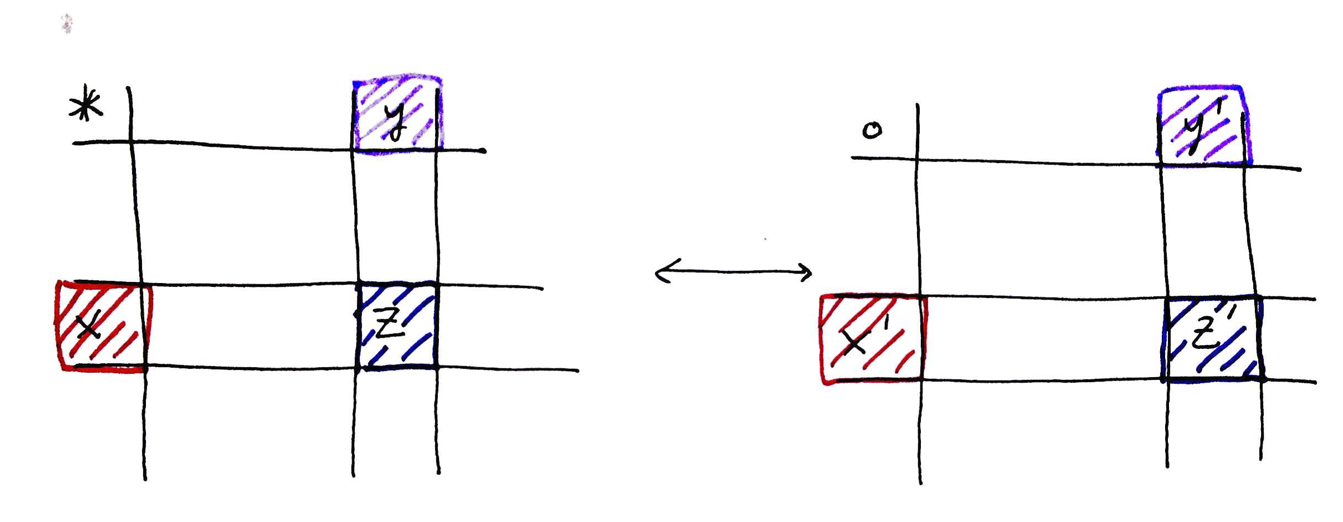
\includegraphics[width=5in]{isoGroupTables.png}
\end{center}

We can describe the isomorphism between $G_1$ and $G_2$ using a function.  Let $\phi:G_1\to G_2$ be the one-to-one and onto function that maps elements of $G_1$ to their corresponding elements in $G_2$.  Then $\phi(x)=x'$, $\phi(y)=y'$, and $\phi(z)=z'$.  Since $z'=x'\circ y'$, we can obtain
\[
\phi(x*y)=\phi(z)=z'=x'\circ y'=\phi(x)\circ \phi(y).
\]
In summary, it must be the case that 
\[
\phi(x*y)=\phi(x)\circ \phi(y).
\]
We are now prepared to state a formal definition of what it means for two groups to be isomorphic.

\begin{definition}\label{def:iso}
Let $(G_1,*)$ and $(G_2,\circ)$ be two groups.  Then $G_1$ is \textbf{isomorphic} to $G_2$, written $G_1\cong G_2$, if and only if there exists a one-to-one and onto function $\phi:G_1\to G_2$ such that
\begin{equation}\label{hom_property}
\phi(x*y)=\phi(x)\circ \phi(y).
\end{equation}
The function $\phi$ is referred to as an \textbf{isomorphism}.  Equation \ref{hom_property} is often referred to as the \textbf{homomorphic property}.
\end{definition}

You should definitely take a few minutes to convince yourself that the above definition agrees with our previous informal approach to isomorphisms.  For those of you that have had linear algebra, notice that our homomorphic property looks a lot like the requirement for a function on vector spaces to be a linear transformation.  Linear transformations preserve the algebraic structure of vector spaces while the homomorphic property is preserving the algebraic structure of groups.

We've seen several instances of two groups being isomorphic, but now that we have a formal definition, we can open the door to more possibilities.

\begin{problem}
Consider the groups $(\mathbb{R},+)$ and $(\mathbb{R}^+,\cdot)$, where $\mathbb{R}^+$ is the set of positive real numbers.  It turns out that these two groups are isomorphic, but this would be difficult to discover using our previous techniques because the groups are infinite.  Define $\phi:\mathbb{R}\to \mathbb{R}^+$ via $\phi(r)=e^r$ (where $e$ is the natural base).
\begin{enumerate}
\item[(a)] Briefly justify why $\phi$ is one-to-one and onto.
\item[(b)] Prove that $\phi$ satisfies the homomorphic property.
\item[(c)] Explain why parts (a) and (b) show that the two groups are isomorphic.
\end{enumerate}
\end{problem}

\begin{exercise}
For each of the following pairs of groups, determine whether the given function is an isomorphism from the first group to the second group.
\begin{enumerate}
\item[(a)] $(\mathbb{Z},+)$ and $(\mathbb{Z},+)$, $\phi(n)=n+1$.
\item[(b)] $(\mathbb{Z},+)$ and $(\mathbb{Z},+)$, $\phi(n)=-n$.
\item[(c)] $(\mathbb{Q},+)$ and $(\mathbb{Q},+)$, $\phi(x)=x/2$.
\end{enumerate}

\end{exercise}

\begin{problem}
Show that the groups $(\mathbb{Z},+)$ and $(2\mathbb{Z},+)$ are isomorphic.
\end{problem}

Perhaps one surprising consequence of the previous problem is that when dealing with infinite groups, a group can have a proper subgroup that it is isomorphic to.  Of course, this never happens with finite groups.

Once we know that two groups are isomorphic, there are lots of interesting things we can say.  The next theorem tells us that isomorphisms map the identity element of one group to the identity of the second group.  It was already clear that this was the case using our informal definition of isomorphic.  Prove the next theorem using Definition~\ref{def:iso}

\begin{theorem}\label{thm:hom_id}
Suppose $\phi:G_1\to G_2$ is an isomorphism from the group $(G_1,*)$ to the group $(G_2,\circ)$.  If $e$ and $e'$ are the identity elements of $G_1$ and $G_2$, respectively, then $\phi(e)=e'$.
\end{theorem}

\begin{theorem}\label{thm:hom_inverse}
Suppose $\phi:G_1\to G_2$ is an isomorphism from the group $(G_1,*)$ to the group $(G_2,\circ)$.   Then $\phi(g^{-1})=[\phi(g)]^{-1}$.
\end{theorem}

\begin{theorem}
Suppose $\phi:G_1\to G_2$ is an isomorphism from the group $(G_1,*)$ to the group $(G_2,\circ)$. If $G_1$ is abelian, then $G_2$ is abelian.
\end{theorem}

\begin{theorem}
Suppose $\phi:G_1\to G_2$ is an isomorphism from the group $(G_1,*)$ to the group $(G_2,\circ)$. Then the function $\phi^{-1}:G_2\to G_1$ is an isomorphism.
\end{theorem}

\begin{theorem}
Suppose $\phi:G_1\to G_2$ and $\psi:G_2\to G_3$ are isomorphisms from the groups $(G_1,*)$ to $(G_2,\circ)$ and $(G_2,\circ)$ to $(G_3,\star)$, respectively. Then the composite function $\psi\circ\phi$ is an isomorphism of $G_1$ and $G_3$.
\end{theorem}

\begin{theorem}
Let $\mathcal{G}$ be any nonempty collection of groups.  Then the relation $\cong$ of being isomorphic is an equivalence relation.
\end{theorem}

\begin{theorem}
Suppose $\phi:G_1\to G_2$ is an isomorphism from the group $(G_1,*)$ to the group $(G_2,\circ)$.  If $H\leq G_1$, then $\phi(H)\leq G_2$, where
\[
\phi(H):=\{y\in G_2:\text{there exists } h\in H\text{ such that }\phi(h)=y\}. 
\]
Note that $\phi(H)$ is called the \textbf{image} of $H$.
\end{theorem}

\begin{theorem}
Suppose $(G,*)$ is a group and let $g\in G$.  Define $\phi_g:G\to G$ via $\phi(x)=g^{-1}xg$.  Then $\phi_g$ is an isomorphism from $G$ to $G$.  Note that the map $\phi_g$ is called \textbf{conjugation} by $g$.
\end{theorem}

Now that you've proved the above theorems, it's a good idea to review the key themes.  If you were really paying attention, you may have noticed that in a few of the proofs, we did not use the fact that the function was one-to-one and onto despite assuming that the function was an isomorphism.

\begin{problem}
For which of the recent theorems could we remove the assumption that the function is one-to-one and onto and only assume that it satisfies the homomorphic property?  Such functions are called \textbf{homomorphisms} and will be the subject of a future chapter.
\end{problem}


\end{section}